\documentclass{article}
\usepackage{scrextend}
\usepackage[dvips,a3paper,centering,margin=2cm]{geometry}
\usepackage{multirow}
\usepackage{framed}
\usepackage{xcolor}
\definecolor{shadecolor}{rgb}{0.2078,0.1098,0.4588}
\usepackage[spanish, english]{babel} 
\usepackage[utf8]{inputenc}
\usepackage{amsmath}
\definecolor{bl}{rgb}{0.2078,0.1098,0.4588}
\definecolor{rb}{rgb}{0.025,0.5,0.9} 
\definecolor{na}{rgb}{0.8274,0.305,0.196} 
\definecolor{ver}{rgb}{1, 0.8627, 0.4078}
\definecolor{ner}{rgb}{0.7568,0.9098,0.9843}
\usepackage{graphicx}  
\pagestyle{empty}
\def\to{\rightarrow}
\begin{document}
\vspace*{-2cm}
\changefontsizes{14pt}
\hspace*{-1cm}
\begin{minipage}{0.2\linewidth}
\vspace{-0.3cm}

\includegraphics[scale=0.2]{images/fcfm.eps}
\end{minipage}
\vspace*{-0.4cm}
\begin{minipage}{0.65\linewidth}
\vspace*{0.7cm}
\begin{center}
\changefontsizes{15pt}
\hspace*{-0.1cm}
\textbf{\textcolor{bl}{Análisis de las irradiancias UVA y Eritémica medidas por el Sistema Monitoreo Atmosférico de la Ciudad de México}}
\end{center}
\vspace{-1cm}
\begin{center}
\changefontsizes{11pt}
Adriana Ipiña$^{*1}$, Gamaliel López$^{2}$, Rubén Piacentini$^{1,3}$\\
1. Instituto de Física Rosario,CONICET-UNR, Argentina\\
2. Facultad de Ciencias Físico-Matemáticas,UANL, México\\
3. Facultad de Ciencias Exactas Ingenieria y Agrimensura, UNR, Argentina\\ *email: ipina@ifir-conicet.gov.ar
\end{center}
\end{minipage}
\begin{minipage}{0.2\linewidth}
\hspace*{0.2cm}
\includegraphics[scale=0.12]{images/ifir.eps}
\end{minipage}\vspace{0.5cm}\\
\changefontsizes{12pt}
\begin{minipage}{0.45\linewidth}
\begin{center}
\begin{shaded}
\textbf{\textcolor{ver}{Introducción}}
\end{shaded}
\end{center}
La Ciudad de México y su área metropolitana (AMCM) es la región más
pobladas de América Latina, así como una de las mayores superficies
urbanas con gran actividad industrial y vehicular.
La radiación solar UV atraviesa la atmósfera interactuando con sus
componentes hasta llegar al suelo. La topografía e inversiones térmicas
en el AMCM, inhiben los vientos que barren los gases y aerosoles de
origen antropogénico. Mediciones en periodos cortos demostraron que
el O$_3$ troposférico reduce cerca del 20\% la intensidad UVB en la
región$^{[1]}$. Otros estudios revelaron que la absorción UV puede atribuirse
a aerosoles orgánicos secundarios producto de la fotoquímica urbana
y/o quema de biomasa$^{[2]}$. Presentamos un análisis de la comparación
con resultados del modelo TUV$^{[3]}$ y mediciones de irradiancia solar UVA
e irradiancia eritémica de 11 estaciones pertenecientes al Sistema de
Monitoreo Atmosférico (SIMAT) del gobierno de la Ciudad de México.\vspace{-0.9cm}\\
\begin{center}
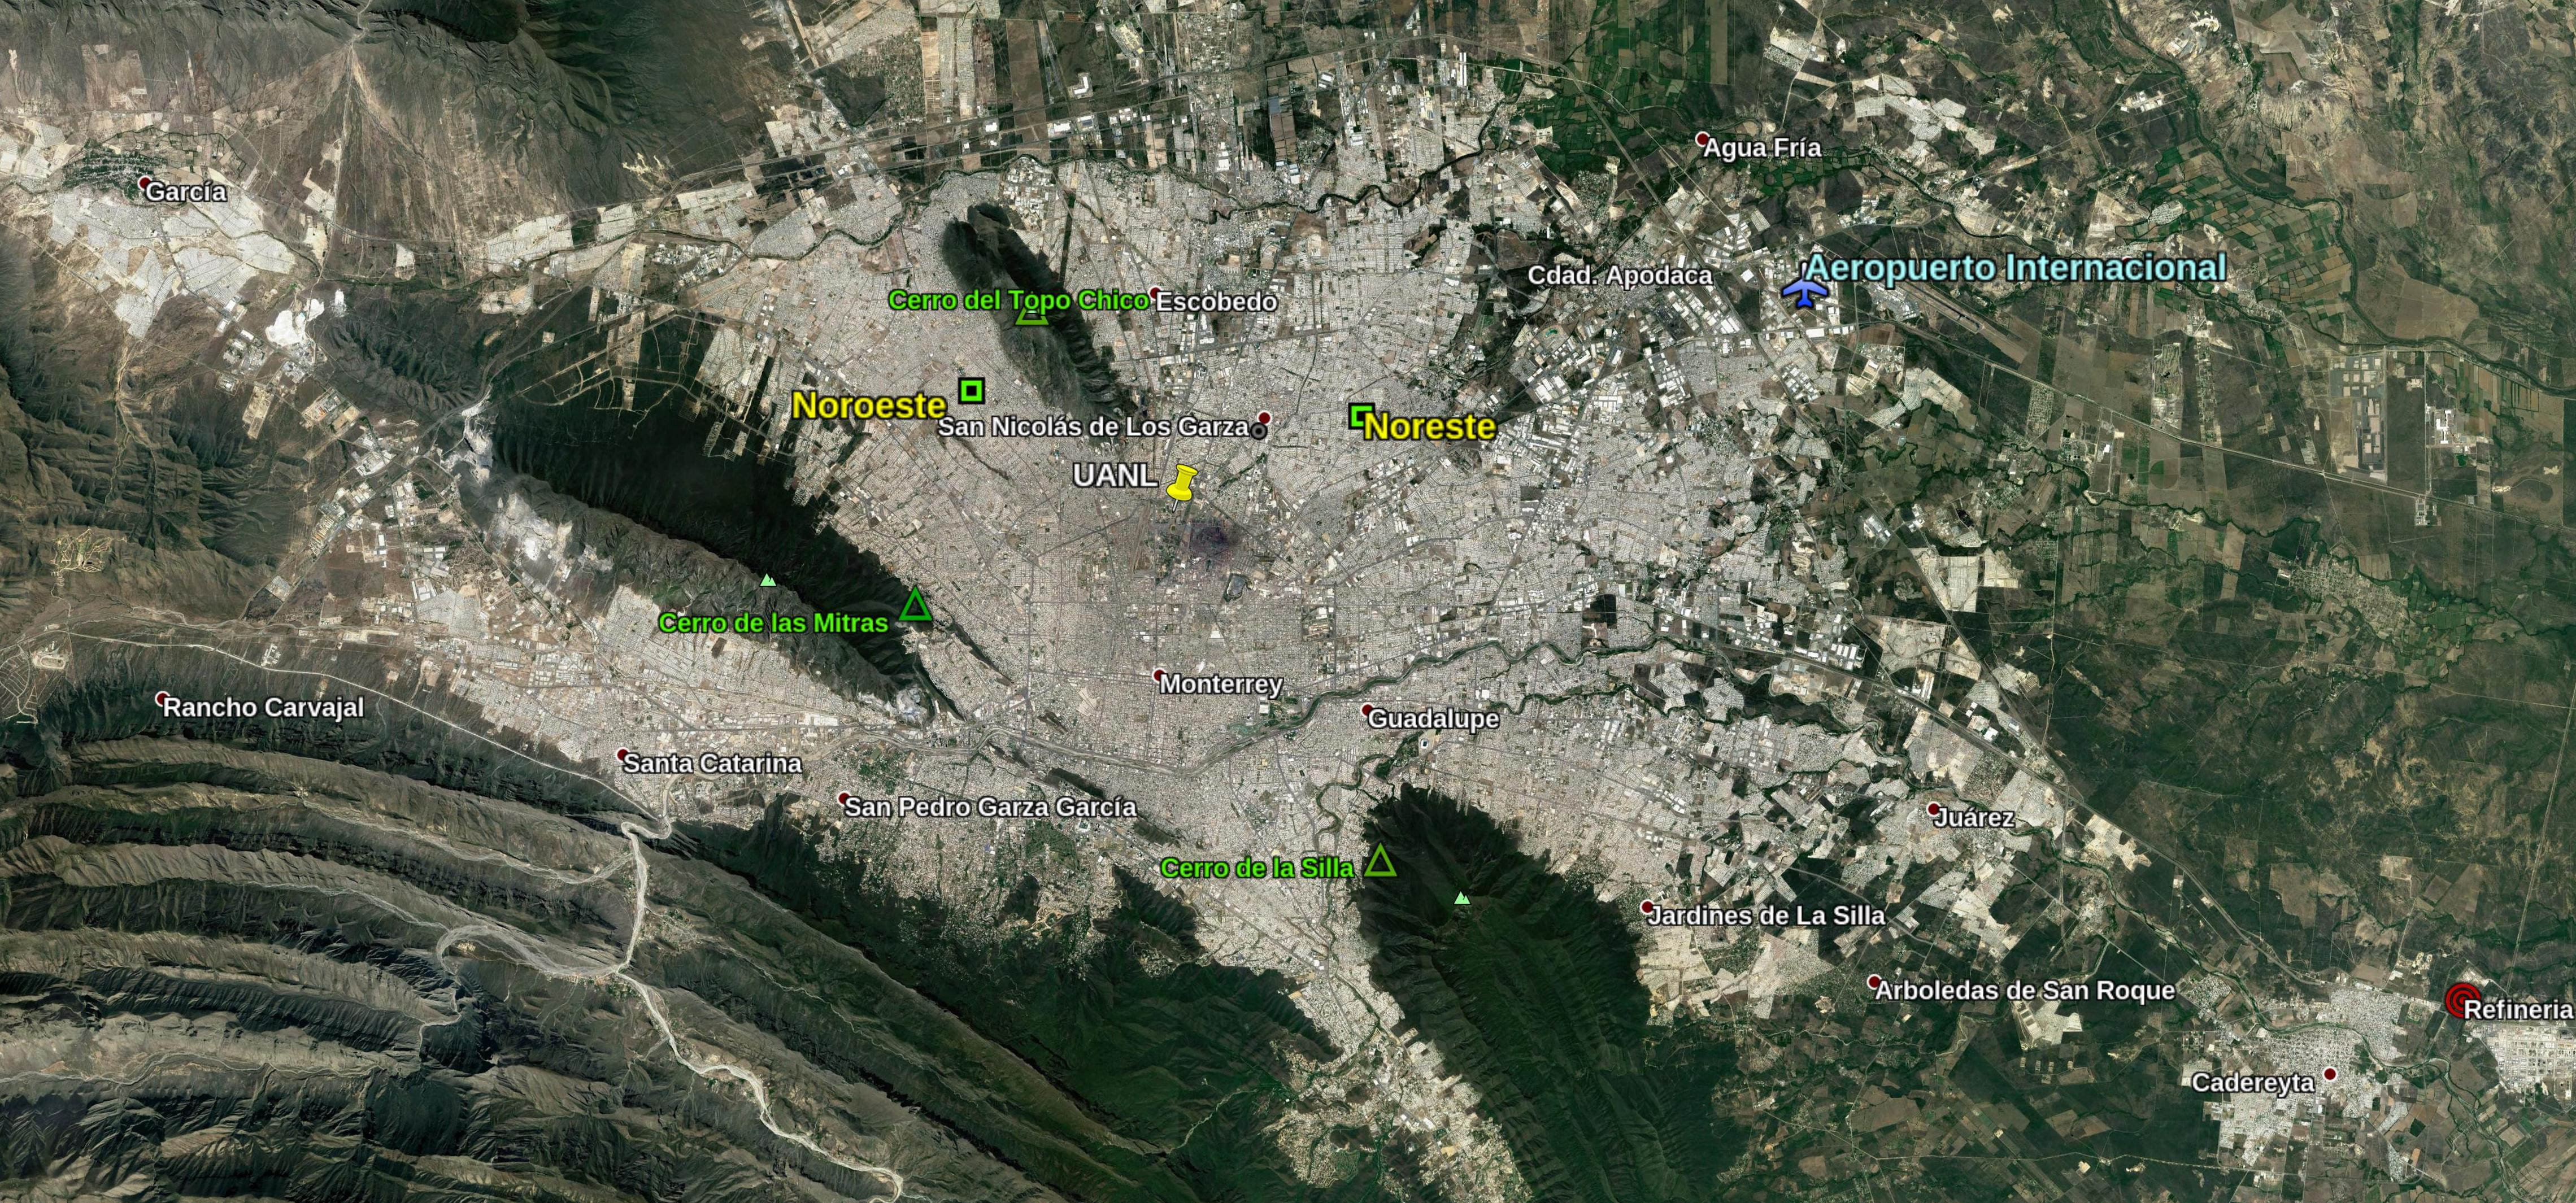
\includegraphics[scale=0.26]{images/satelite.eps}\\
\changefontsizes{9.5pt}
\textcolor{bl}{Ubicación de las estaciones del SIMAT en el AMCM y principales volcanes}
\end{center}
\end{minipage}
\hspace{0.7cm}
\begin{minipage}{0.53\linewidth}
\vspace{-0.16cm}
\begin{center}
\begin{shaded}
\textbf{\textcolor{ver}{Metodologia}}
\end{shaded}
\vspace{-0.7cm}
\end{center}
\begin{minipage}{0.5\linewidth}
\begin{center}
\colorbox{ner}{\changefontsizes{9pt} \hspace{3.07cm}Merced (MER)\hspace{3.07cm}\vspace{0.3cm}}\vspace{0.2cm}\\
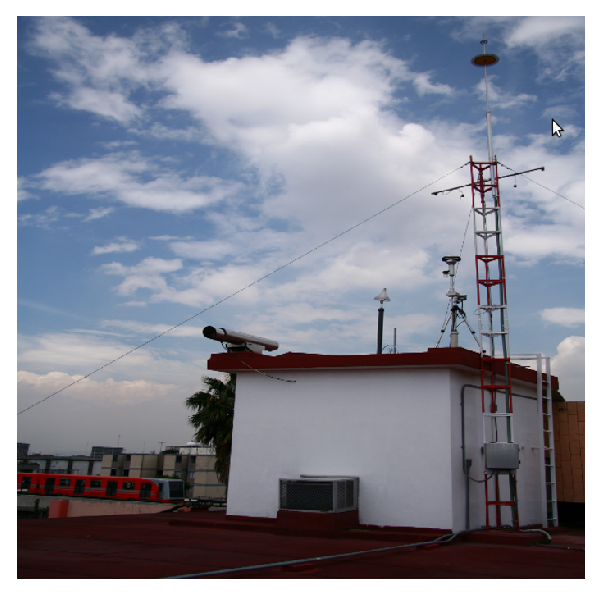
\includegraphics[scale=0.745]{images/mer.eps}
\end{center}
\end{minipage}
\hspace{0.1cm}
\begin{minipage}{0.23\linewidth}
\colorbox{ner}{\changefontsizes{9pt} \hspace{0.3cm} Noroeste(NO) \hspace{0.3cm}}

\includegraphics[scale=0.68]{images/noroeste.eps}\\
\colorbox{ner}{\changefontsizes{9pt} \hspace{0.4cm} Suroeste(SO) \hspace{0.4cm}}

\includegraphics[scale=0.68]{images/suroeste.eps}
\end{minipage}
\begin{minipage}{0.23\linewidth}
\colorbox{ner}{\changefontsizes{9pt} \hspace{0.4cm} Noreste(NE) \hspace{0.4cm}}

\includegraphics[scale=0.68]{images/noreste.eps}\\
\colorbox{ner}{\changefontsizes{9pt} \hspace{0.5cm} Sureste(SE)   \hspace{0.5cm}}

\includegraphics[scale=0.68]{images/sureste.eps}
\end{minipage}
\changefontsizes{9pt}
\textcolor{bl}{Estación meteorológica Merced (MER) e imágenes en 4 orientaciones}\\
\changefontsizes{12pt}
Se filtraron mediciones bajo cielo despejado minuto a minuto de las
irradiancia solar UVA y eritémica para el año 2016 en la estación MER,
utilizando esas fechas como referencia. Se modificó el código fuente del
modelo TUV para introducir la ubicación geográfica de cada estación
[lat, lon, a.s.n.m.] del SIMAT y los principales valores de entrada
\begin{center}
\changefontsizes{8.5pt}
\begin{tabular}{|c|c|c|c|c|c|} \hline
Reflectividad & & & Exponente & Albedo de &  \\
del suelo &O$_3$ col DU &N0$_2$ col DU &de Angstrom &  dispersión simple &AOD$_{500}$ \\
& & && de aerosol&  \\ \hline
0.06 & Medición satelital & 0.1 & 1 & 0.80$^{[2]}$ & AERONET$^{[5]}$ \\
& OMI-NASA$^{[4]}$ & &&& \\ \hline
\end{tabular}
\end{center}
Se tomó el promedio diario de AOD$_{500nm}$ (de la red AERONET) medido
en la estación del Centro de Ciencias de la Atmósfera (CCA-UNAM).
Finalmente se calculó la razón (R) ModeloTUV/Medición, al mediodía
solar para ambas irradiancias y cada estación que contaba con datos.
\end{minipage}
\begin{center}
\begin{shaded}
\textbf{\textcolor{ver}{Resultados}}
\end{shaded}
\end{center}
\begin{minipage}{0.52\linewidth}
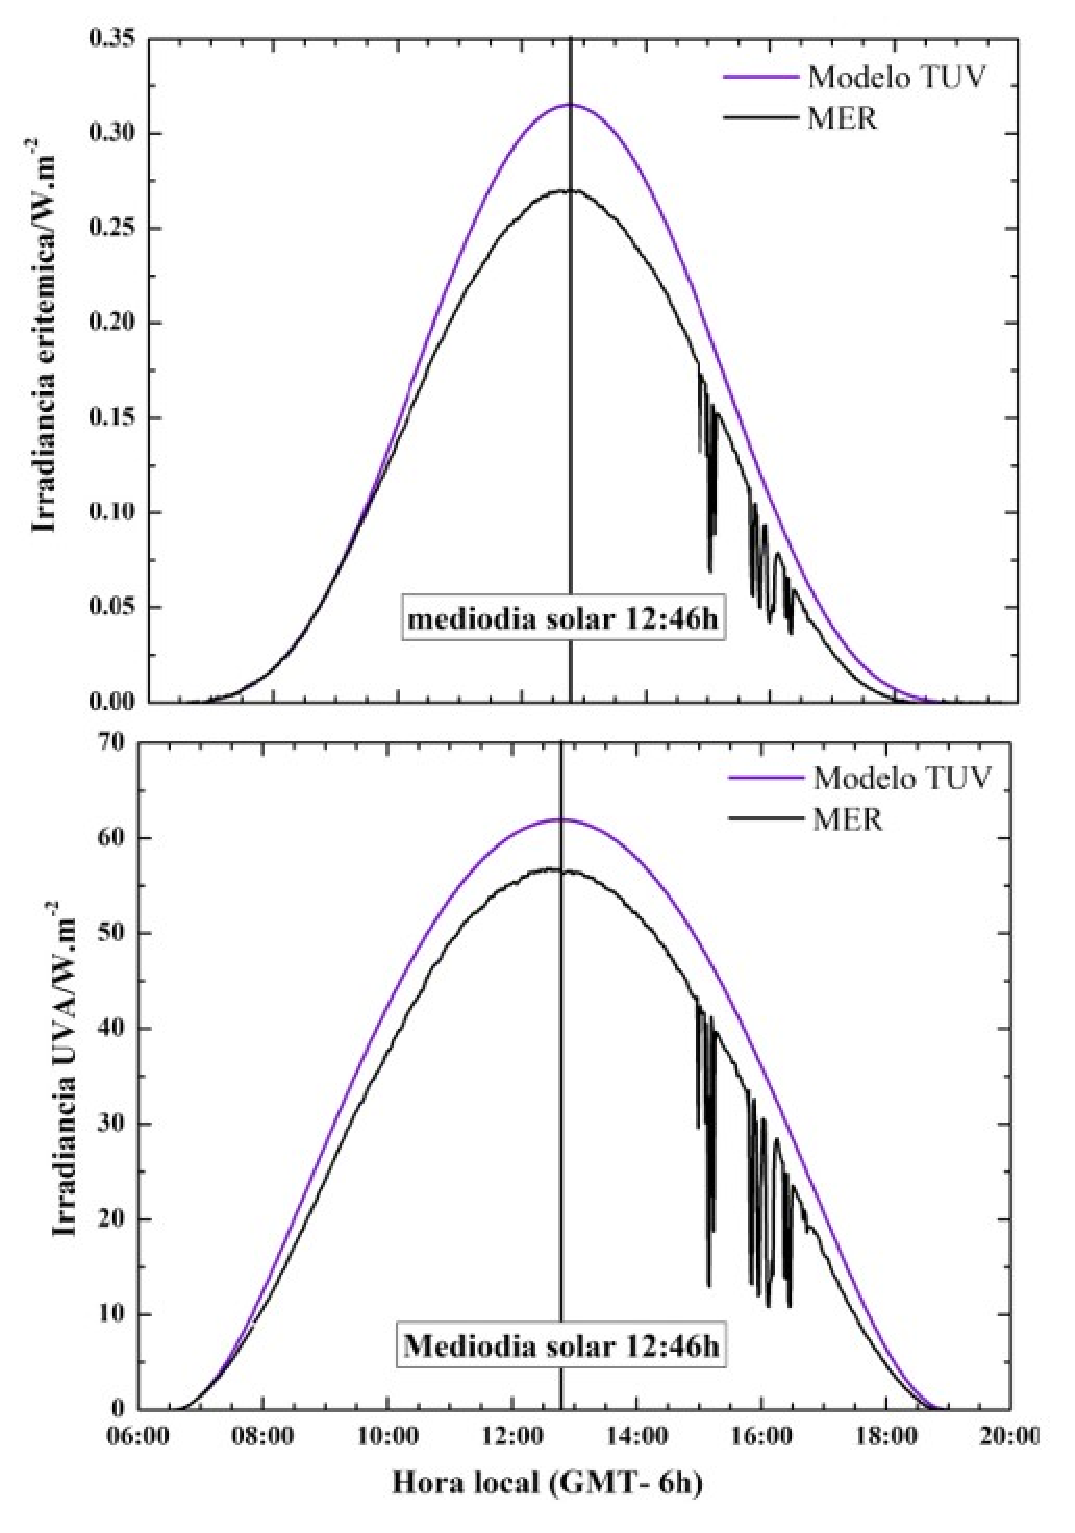
\includegraphics[scale=0.4]{images/espectro.eps}
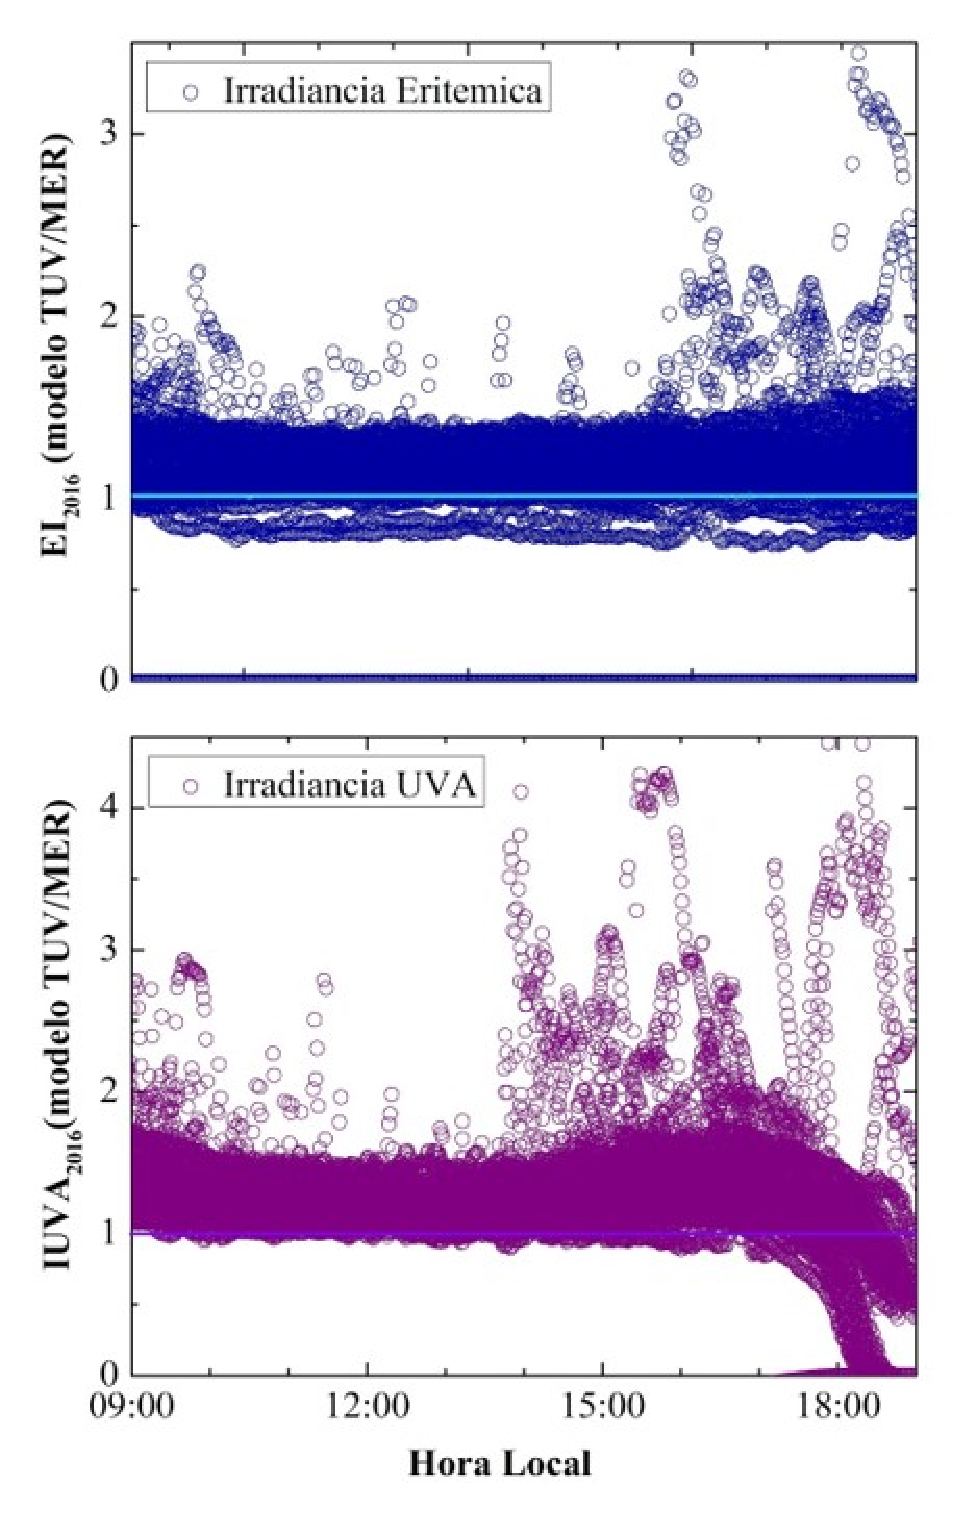
\includegraphics[scale=0.4]{images/uvaanual.eps}\\
\changefontsizes{9.5pt}
\textcolor{bl}{Irradiancia solar eritémica e irradiancia solar UVA: medición y modelo TUV minuto a minuto el día 11/Mar/2016 (izq). R$_{Eri}$ y R$_{UVA}$ minuto a minuto
para todos los días de medición bajo cielo despejado del 2016 (der).}
\end{minipage}
\begin{minipage}{0.46\linewidth}
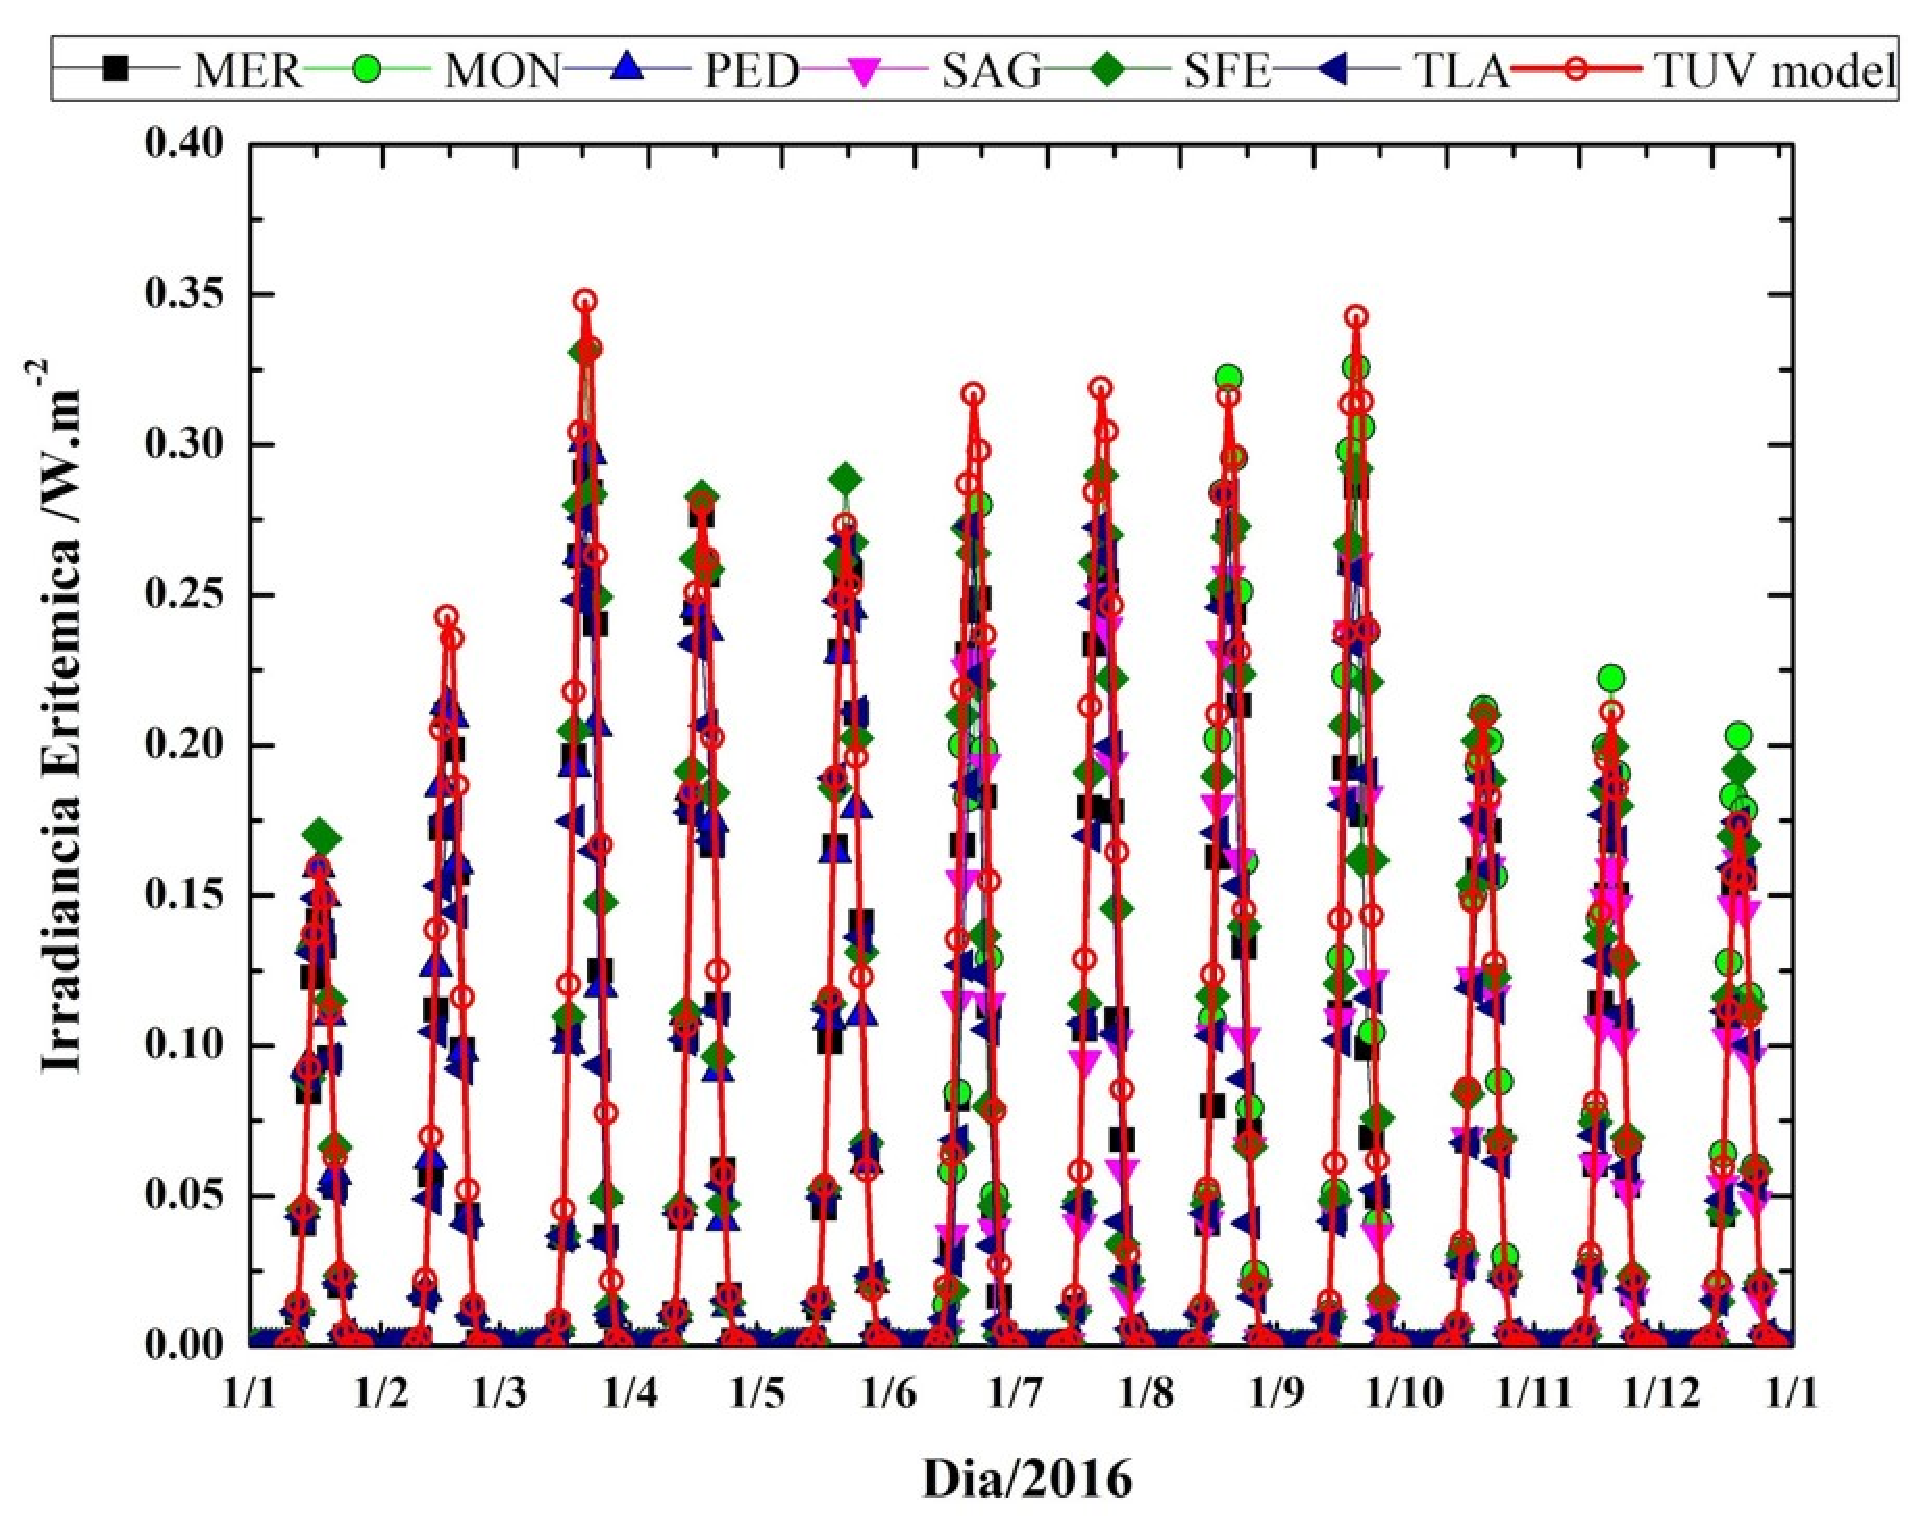
\includegraphics[scale=0.4]{images/erydia.eps}\\
\changefontsizes{9.5pt}
\textcolor{bl}{Irradiancia eritémica: medida y calculada con modelo TUV cada hora.
Representación mes a mes del año 2016 para un día de cielo}
\end{minipage}\vspace{0.1cm}\\
\begin{minipage}{0.50\linewidth}
\begin{center}
\begin{shaded}
\textbf{\textcolor{ver}{Conclusiones}}
\end{shaded}
\end{center}
\vspace{-0.85cm}
\begin{itemize}
    \item La topografía e inmersión térmica influyen en el aerosol debajo
de la capa límite y por tanto en la irradiancia UVA y eritémica.
    \item Filtrar las mediciones minuto a minuto en días despejados para
comparar con el modelo TUV facilita la adecuada selección.
\item El promedio de las R al mediodia solar de las irradiancias UVA y
eritémica son: R$_{UVA}$=1.16 y R$_{Eri}$ =1.14 respectivamente, para
todos los días medidos en cielo despejado del año 2016.
\end{itemize}
\end{minipage}
\hspace{1cm}\vspace{0.5cm}
\begin{minipage}{0.45\linewidth}
\begin{center}
\begin{shaded}
\textbf{\textcolor{ver}{Referencias}}
\end{shaded}
\end{center}
\changefontsizes{9pt}
\vspace{-0.7cm}
\begin{enumerate}
\bibitem[1]{Acosta} Acosta LR, Evans WFJ. J. Geophysical Research (105) 5017–5026 2000.
\bibitem[2]{Palancar} G. G. Palancar et al. 2013 Atmos. Chem. Phys., (13) 1011–1022, 2013.
\bibitem[3]{Madronich} S. Madronich, Environ. UV Photob. 1–39, 1993.
\bibitem[4]{Torres} Torres O, OMI/Aura Near-UV AODV3, NASA Goddard Space Flight Center, Goddard
Earth Sciences Data and Information Services Center (GES DISC) 2008.
\bibitem[5]{Aeronet} AERONET Network https://aeronet.gsfc.nasa.gov/
\end{enumerate}
\end{minipage}
\end{document}